\documentclass[a4paper]{report}

%====================== PACKAGES ======================

\usepackage[french]{babel}
\usepackage[utf8x]{inputenc}
%pour gérer les positionnement d'images
\usepackage{float}
\usepackage{amsmath}
\usepackage{graphicx}
\usepackage[colorinlistoftodos]{todonotes}
\usepackage{url}
%pour les informations sur un document compilé en PDF et les liens externes / internes
\usepackage{hyperref}
%pour la mise en page des tableaux
\usepackage{array}
\usepackage{tabularx}
%pour utiliser \floatbarrier
%\usepackage{placeins}
%\usepackage{floatrow}
%espacement entre les lignes
\usepackage{setspace}
%modifier la mise en page de l'abstract
\usepackage{abstract}
%police et mise en page (marges) du document
\usepackage[T1]{fontenc}
\usepackage[top=2cm, bottom=2cm, left=2cm, right=2cm]{geometry}
%Pour les galerie d'images
\usepackage{subfig}

\usepackage{tikz}
\usetikzlibrary{arrows,positioning}


%%%%%%
\usepackage{pgf-umlcd}
\usepackage[T1]{fontenc}
\usepackage[utf8x]{inputenc}
\usepackage[french]{babel}
\usepackage{fullpage}
%%%%%%

%%%%%%%%%%%%%%%%%
\usepackage[T1]{fontenc}
\usepackage[utf8x]{inputenc}
\usepackage[french]{babel}
\usepackage{fullpage}

\usepackage{tikz-uml}

\sloppy
\hyphenpenalty 10000000
%%%%%%%%%%%%%%%%%

%%%%%
\usepackage{hyperref}%for \hypersetup
\hypersetup
{
    pdfauthor={Wangyan Li liwangyan618907@gmail.com},
    pdfsubject={tikz, structure},
    pdftitle={The architecture of the consensus filtering algorithm},
    pdfkeywords={tikz, structure}
}

\usepackage{verbatim}
\usepackage{forest}
\usetikzlibrary{arrows.meta, shapes.geometric, calc, shadows,fit}

\colorlet{mygreen}{green!75!black}
\colorlet{col1in}{red!30}
\colorlet{col1out}{red!40}
\colorlet{col2in}{mygreen!40}
\colorlet{col2out}{mygreen!50}
\colorlet{col3in}{blue!30}
\colorlet{col3out}{blue!40}
\colorlet{col4in}{mygreen!20}
\colorlet{col4out}{mygreen!30}
\colorlet{col5in}{blue!10}
\colorlet{col5out}{blue!20}
\colorlet{col6in}{blue!20}
\colorlet{col6out}{blue!30}
\colorlet{col7out}{orange}
\colorlet{col7in}{orange!50}
\colorlet{col8out}{orange!40}
\colorlet{col8in}{orange!20}
\colorlet{linecol}{blue!60}

%%%%%
%====================== INFORMATION ET REGLES ======================

%rajouter les numérotation pour les \paragraphe et \subparagraphe
\setcounter{secnumdepth}{4}
\setcounter{tocdepth}{4}

\hypersetup{							% Information sur le document
pdfauthor = {Chaar Ismail,
			Mahmoud Lamrani,
			},			% Auteurs
pdftitle = {Projet Java EE -
			Réalisation d'une E-boutique de livre},			% Titre du document
pdfsubject = {Rapport de Projet},		% Sujet
pdfkeywords = {Tag1, Tag2, Tag3, ...},	% Mots-clefs
pdfstartview={FitH}}					% ajuste la page à la largueur de l'écran
%pdfcreator = {MikTeX},% Logiciel qui a crée le document
%pdfproducer = {}} % Société avec produit le logiciel

%======================== DEBUT DU DOCUMENT ========================

\begin{document}

%régler l'espacement entre les lignes
\newcommand{\HRule}{\rule{\linewidth}{0.5mm}}

%page de garde
\begin{titlepage}
\begin{center}

% Upper part of the page. The '~' is needed because only works if a paragraph has started.

\includegraphics[width=0.35\textwidth]{./logo}~\\[1cm]

\textsc{\LARGE L'Ecole Nationale Supérieure d'Informatique et d'Analyse des Systèmes}\\[1.5cm]

\textsc{\Large }\\[0.5cm]

% Title
\HRule \\[0.4cm]

{\huge \bfseries Projet Java EE\\
Réalisation d'une E-boutique de livre \\[0.4cm] }

\HRule \\[1.5cm]

% Author and supervisor
\begin{minipage}{0.4\textwidth}
\begin{flushleft} \large
\emph{Réalisé par:}\\
Ismail \textsc{Chaar}\\
Mahmoud \textsc{Lamrani}\\

\end{flushleft}
\end{minipage}
\begin{minipage}{0.4\textwidth}
\begin{flushright} \large
\emph{Encadré par:} \\
Mr. Mahmoud \textsc{EL HAMLAOUI}\\

\end{flushright}
\end{minipage}

\vfill

% Bottom of the page


\end{center}
\end{titlepage}

%page blanche
\newpage
~
%ne pas numéroter cette page
\thispagestyle{empty}
\newpage

\renewcommand{\abstractnamefont}{\normalfont\Large\bfseries}
%\renewcommand{\abstracttextfont}{\normalfont\Huge}

\begin{abstract}
\hskip7mm

\begin{spacing}{1.3}
Des ventes de main en main, vers des ventes virtuelles, passent les priorités des opérations de ventes des biens et des services, ce qui nous rend obligés à donner plus d’importance à la vente électronique.
Les boutiques en ligne sont depuis des années, largement conseillées pour les entreprises qui se basent sur la vente des produits, et même des services. Ces types de sites web représentent un dispositif global fournissant aux clients un pont de passage à l’ensemble des informations, des produits, et des services à partir d’un portail unique en rapport avec son activité.
Les sites de vente en ligne permettant aux clients de profiter d’une foire virtuelle disponible sont quotidiennement mises à jour sans la moindre contrainte, ce qui leur permettrait de ne jamais rater les coups de cœur, ainsi une foire sans problème de distance géographique, ni d’horaire de travail ni de disponibilité de transport. D’une autre par ces sites offre à l'entreprise de profiter de cet espace pour exposer ses produits à une plus large base de clientèle.
Notre projet est de réaliser dans le cadre du projet java EE de deuxième année GL ayant comme objectif principal : la conception et la réalisation d'une E-boutique de livre. Ce rapport est composé de trois volets, le premier contient le cahier de charges. Dans le deuxième, nous décrivons l’analyse et la conception de notre application, et dans le troisième nous présentons les outils utilisés pour la réalisation ainsi que des captures d’écran de l’application avec description.
\end{spacing}
\end{abstract}


\tableofcontents
\thispagestyle{empty}
\setcounter{page}{0}
%ne pas numéroter le sommaire

\newpage

%espacement entre les lignes d'un tableau
\renewcommand{\arraystretch}{1.5}

%====================== INCLUSION DES PARTIES ======================

~
\thispagestyle{empty}
%recommencer la numérotation des pages à "1"
\setcounter{page}{0}
\newpage



\chapter{Présentation du projet}

Aujourd’hui, le commerce électronique est considéré comme un dossier prioritaire par de nombreuses organisations internationales . L'objectif de notre projet est le développement d’un site web d’e-commerce afin de gérer un ensemble de tâches facilitant l’achat de livre en ligne sans se déplacer sur place.
%note en bas de page

\section{Analyse du Sujet}




\begin{figure}[H]
    \centering
\scalebox{0.70}{
\begin{forest}
 for tree={
  font=\sffamily\bfseries,
  line width=1pt,
  draw=linecol,
  ellip,
  align=center,
  child anchor=north,
  parent anchor=south,
  drop shadow,
  l sep=1cm,
  edge path={
    \noexpand\path[color=linecol, rounded corners=5pt,
      >={Stealth[length=10pt]}, line width=1pt, ->, \forestoption{edge}]
      (!u.parent anchor) -- +(0,-5pt) -|
      (.child anchor)\forestoption{edge label};
    },
  where level={3}{tier=tier3}{},
  where level={0}{l sep-=15pt}{},
  where level={1}{
    if n={1}{
      edge path={
        \noexpand\path[color=linecol, rounded corners=5pt,
          >={Stealth[length=10pt]}, line width=1pt, ->,
          \forestoption{edge}]
          (!u.south) --++(0,-8pt) -| (.child anchor)\forestoption{edge label};
        },
    }{
      edge path={
        \noexpand\path[color=linecol, rounded corners=5pt,
          >={Stealth[length=10pt]}, line width=1pt, ->,
          \forestoption{edge}]
          (!u.south) --++(0,-8pt) -| (.child anchor)\forestoption{edge label};
        },
     }
    }{},
  }
   [Les Cmds des clients sur l'E-boutique,l sep=1.5cm, outer color=col3out
    [Reception de la Cmd 1,name=sensor1,
    [validation manuelle de la Cmd 1, rect, name=sse1
    ]
  ]
  [Reception de la Cmd 2,name=sensor2,
    [validation manuelle de la Cmd 2, rect, name=sse2
    ]
  ]
  [, phantom, calign with current
    [A\\B, phantom
      [Livraison des commandes aux clients, orect, name=us
        [{Clients satisfaits}, oellip
        ]
      ]
    ]
  ]
  [Reception de la Cmd N-1,name=sensor3,
    [validation manuelle de la Cmd N-1, rect, name=sse3
    ]
  ]
  [Reception de la Cmd N,name=sensor4,
    [validation manuelle de la Cmd N, rect, name=sse4
    ]
  ]
]
  \begin{scope}[color = linecol, rounded corners = 5pt,
    >={Stealth[length=10pt]}, line width=1pt, ->]
    \draw (sse2.south) -- (us.north -| sse2.south);
    \draw (sse3.south) -- (us.north -| sse3.south);
    \coordinate (c1) at ($(sse1.south)!2/5!(sse2.south)$);
    \coordinate (c2) at ($(sse3.south)!3/5!(sse4.south)$);
    \draw (sse1.south) -- +(0,-22pt) -| (us.north -| c1);
    \draw (sse4.south) -- +(0,-22pt) -| (us.north -| c2);
    \node[draw,dash dot,fit=(sensor1)(sse4)(sensor4),inner ysep=12pt,]{};
    \coordinate (m1) at ($(sse2)!0.5!(sensor2)$);
    \coordinate (m2) at ($(sensor2)!0.5!(sensor3)$);
    \node[scale=3] at (m1-|m2) {...};
  \end{scope}
\end{forest}}
    \caption{Schéma descriptif}
\end{figure}





La procédure de passage des livres de la boutique vers les mains du client via l'E-boutique est la suivante :

Le client choisit les livres qu'il veut ainsi que la quantité et ensuite passe sa commande.
Le gestionnaire du site marchand valide la commande de cet internaute et transmet tous les éléments au livreur. 
Le livreur prépare la commande et réalise les expéditions.

\newpage

\section{Étude de l'existant}

Pour acheter un livre, le client doit se déplacer directement au local de la boutique de livre. Ses déplacements peuvent être inutiles, et même peuvent provoquer un gaspillage de temps. D’ailleurs, même le vendeur n’a aucun moyen pour mettre à disposition ses annonces de vente et services, à l’exception des supports traditionnels tels que les journaux ou les petites affiches. Ainsi, un moyen fiable et automatisé permettant d’informer un grand nombre de clients des offres de vente et des services nécessaires. Divers autres traitements sont, d’ailleurs, sources de problèmes, adoptant les méthodes traditionnelles de travail :

\begin{itemize}
\item Le règlement des factures se fait en espèce ou par chèque, sur place. 
\item L’enregistrement des clients se fait manuellement sur papier. 
\item Les livres sont classés par des catégories non liées et non hiérarchisées, ce qui rend la recherche plus pénible.
\end{itemize}



\section{Solutions proposées}

%Quoi :
Grâce à Internet, de nouvelles perspectives de développement apparaissent dans l'élargissement du marché économique.

La création d’un site Internet a pour but de valoriser l'image de la société et faire des économies. L'utilisation d'Internet, comme segment de communication de masse, permet également de baisser des coûts marketing et d'autres frais. Avec la transmission du haut débit et la sécurisation augmentée des moyens sécurisés de paiement, la confiance des utilisateurs en ce qui concerne l'e-commerce est croissante. La plupart des personnes adultes utilisent, aujourd’hui, Internet pour faire des achats. Les consommateurs et les entreprises s'orientent de plus en plus vers les boutiques en ligne qui permettent la comparaison, la disponibilité des produits et la vérification des prix d’où l’économie considérable du temps.
\bigbreak
Ce projet consiste donc à la mise en place d’un site Web dynamique qui gère la commercialisation de livres. Ceci est possible à travers des catalogues en ligne. Les clients peuvent consulter le site et commander des livres après une inscription, qui sont par la suite livrés à domicile.\\

Cette boutique en ligne permettra d’offrir beaucoup des services à savoir :
\begin{itemize}
\item Recherche de livre,
\item Consultation de catégories de livre,
\item Lancer une commande en ligne,
\end{itemize}
\bigbreak
Cette application Web permettra de cibler une nouvelle catégorie de clientèles , et d’offrir une meilleure qualité de service en communication et en commerce. Ce site devra contenir deux interfaces séparées :\\

Partie administrateur du site : l’administrateur du site doit s’authentifier avec son login et son mot de passe à partir de la page d’accueil. Après son authentification comme administrateur, il pourra accéder à la page qui lui permettra de gérer les outils d’administration. Le site affichera toutes les tâches qui peuvent être effectuées par l’administrateur qui pourra:

\begin{itemize}
\item Ajouter un livre : chaque livre est caractérisé par son nom et sa catégorie.
\item Gérer des comptes : ajout ou suppression d’un compte. Chaque compte est caractérisé par le login, le mot de passe, le nom, le prénom et l'adresse du client.
\item Déconnexion : cela permet la sécurité de l’interface.
\end{itemize}
\bigbreak
Partie client : cette interface doit être accessible à n’importe quel internaute cherchant des livres et effectuant des commandes.

%Detail :
%%Bla(cf. ref. \cite{cite6}).
%citation référencé dans le document "bibliographie.bib" inclus à la fin du document



\chapter{Analyse et conception}

On expose, dans ce chapitre, la solution conceptuelle qu'on a proposée et cette conception du système à réaliser qui a pour but de rendre flexible la tâche de la gestion. En d’autre terme, ce chapitre devrait répondre à la question : comment faire ? La structure de ce chapitre dépend de la nature de ce projet. la phase de conception d’un système d’information nécessite des méthodes permettant de mettre en place un modèle. pour en faire on a utilisé le Langage de Modélisation Unifié, de l'anglais Unified Modeling Language UML, qui est un langage de modélisation graphique conçu pour fournir une méthode normalisée pour visualiser la conception d'un système. Il est couramment utilisé en développement logiciel et en conception orientée objet.

\section{Le diagramme du cas d’utilisation}

Le rôle des diagrammes de cas d’utilisation est de recueillir, d’analyser et d’organiser les besoins, ainsi que de recenser les grandes fonctionnalités d’un système. Il s’agit donc de la première étape UML pour la conception d’un système.

\subsection{Les composants d'un diagramme de cas d'utilisation}

Le diagramme de cas se compose de trois éléments principaux :
\bigbreak
\begin{itemize}
\item Un Acteur : c’est l’idéalisation d’un rôle joué par une personne externe, un processus ou une chose qui interagit avec un système. Il se représente par un petit bonhomme avec son nom inscrit dessous.
\item Un cas d’utilisation : c’est une unité cohérente représentant une fonctionnalité visible de l’extérieur. Il réalise un service de bout en bout, avec un déclenchement, un déroulement et une fin, pour l’acteur qui l’initie.
\item Une relation : trois types de relations sont pris en charge par la norme UML et sont graphiquement représentés par des types particuliers de ces relations. Les relations indiquent que le cas d'utilisation source présente les mêmes conditions d'exécution que le cas issu. Une relation simple entre un acteur et une utilisation est un trait simple.
\end{itemize}


\subsection{Diagramme de cas d’utilisation du projet}

\begin{figure}[H]
\centering
\scalebox{0.99}{
\begin{tikzpicture}
\begin{umlsystem}[x=4, fill=red!10]{E-boutique de livre} 
  \umlusecase[name=case1,x=3]{consulter livres}
  \umlusecase[name=case13,x=3,y=-1]{creer un compte} 
  \umlusecase[name=case2,x=3,y=-2.7, width=1.7cm]{ajouter des livres au panier}
  \umlusecase[name=case3,x=3,y=-4.7, fill=green!20]{s'authentifier}
  \umlusecase[name=case7,y=-7]{enregistrer panier}
  \umlusecase[name=case8,y=-9, width=2cm]{passer commande}
  \umlusecase[name=case9,y=-11, width=2cm]{consulter ses commandes}
  \umlusecase[name=case6,x=6, y=-7]{gerer les categories}
  \umlusecase[name=case10,x=6, y=-8.5]{gerer les livres}
  \umlusecase[name=case11,x=6, y=-10]{gerer les clients}
  \umlusecase[name=case12,x=6, y=-11.5]{gerer les commandes}

\end{umlsystem}

\umlactor{visiteur} 
\umlactor[y=-6.5]{client} 
\umlactor[x=14.5, y=-6.5]{administrateur}

\umlinherit{client}{visiteur}
\umlassoc{visiteur}{case1}
\umlassoc{visiteur}{case2} 
\umlassoc{visiteur}{case13}
\umlassoc{client}{case3}
\umlassoc{client}{case7}
\umlassoc{client}{case8} 
\umlassoc{client}{case9} 
\umlassoc{administrateur}{case3} 
\umlassoc{administrateur}{case6}
\umlassoc{administrateur}{case10}
\umlassoc{administrateur}{case11}
\umlassoc{administrateur}{case12}

\umlinclude[name=incl]{case7}{case3}
\umlinclude[name=incl]{case8}{case3}
\umlinclude[name=incl]{case9}{case3}
\umlinclude[name=incl]{case6}{case3}
\umlinclude[name=incl]{case10}{case3}
\umlinclude[name=incl]{case11}{case3}
\umlinclude[name=incl]{case12}{case3}

\end{tikzpicture}}
\caption{Diagramme de cas d'utilisation de l'E-boutique de livre}
\end{figure}


\section{Les diagrammes de séquences}

Un diagramme de séquences est un diagramme d'interaction qui expose en détail la façon dont les opérations sont effectuées : quels messages sont envoyés et quand ils le sont.

\subsection{Le modèle MVC}
En ce qui suit, nous présenterons quelques diagrammes de séquences relatifs aux cas d’utilisations présentes.
Les diagrammes de séquences sont basés sur le modèle MVC :
\begin{figure}
    \centering
    \begin{tikzpicture}[node distance=1cm, auto]  
\tikzset{
    mynode/.style={rectangle,rounded corners,draw=black, top color=white, bottom color=yellow!50,very thick, inner sep=1em, minimum size=3em, text centered},
    myarrow/.style={->, >=latex', shorten >=1pt, thick},
    mylabel/.style={text width=7em, text centered} 
}  
\node[mynode] (Model) {Model};  
\node[below=3cm of Model] (dummy) {}; 
\node[mynode, left=of dummy] (View) {View};  
\node[mynode, right=of dummy] (Controler) {Controler};

% The text width of 7em forces the text to break into two lines. 

\draw[myarrow] (Model.west) -- ++(-0,0) -- ++(0,0) -|  (View.north);	
\draw[myarrow] (Controler.north) -- ++(0,1) -- ++(0,0) |-  (Model.east);
\draw[myarrow] (Controler.west) -- ++(0,0) -- ++(0,0) --  (View.east);
% There is a slight overlap of the arrows with the (Model) south edge
% because creating the offset in another way didn't compile. 
 

% The swap command corrects the placement of the text.

\end{tikzpicture} 
    \caption{L'architecture MVC}
    
\end{figure}

\begin{itemize}
\item Modèle : cette partie gère les données du site. Son rôle est d'aller récupérer les informations « brutes » dans la base de données, de les organiser et de les assembler pour qu'elles puissent ensuite être traitées par le contrôleur. On y trouve donc entre autres les requêtes SQL.
\item Vue : cette partie se concentre sur l'affichage. Elle ne fait presque aucun calcul et se contente de récupérer des variables pour savoir ce qu'elle doit afficher. On y trouve essentiellement du code HTML mais aussi quelques boucles et conditions très simples, pour afficher par exemple une liste de messages.
\item Contrôleur : cette partie gère la logique du code qui prend des décisions. C'est en quelque sorte l'intermédiaire entre le modèle et la vue : le contrôleur va demander au modèle les données, les analyser, prendre des décisions et renvoyer le texte à afficher à la vue. Le contrôleur contient exclusivement du code Java. C'est notamment lui qui détermine si le visiteur a le droit de voir la page ou non (gestion des droits d'accès).
\end{itemize}


\subsection{Diagrammes de séquences du projet}

\begin{figure}[H]
    \centering
    \begin{tikzpicture}
\begin{umlseqdiag}
\umlactor[no ddots]{Visiteur}
\umlboundary[class=Vue, fill=blue!20]{FenetreAuth}
\umlcontrol[class=Controleur,x=8.5, fill=blue!20]{ServletConnexion}
\umlentity[class=Modele,x=13, fill=blue!20]{ClientDAO}

\begin{umlcall}[op=SaisirInformation(), type=synchron]{Visiteur}{FenetreAuth}
\begin{umlcallself}[op=VerificationChamps(), type=synchron]{FenetreAuth}
\end{umlcallself}
\begin{umlcall}[op=EnvoyerInfo(), type=synchron]{FenetreAuth}{ServletConnexion}
\begin{umlcall}[op=EnvoyerInfo(string\,String), type=synchron,return=Afficher()]{ServletConnexion}{ClientDAO}
\begin{umlcallself}[op=VerifiInfos(), type=synchron]{ClientDAO}
\end{umlcallself}
\end{umlcall}
\begin{umlfragment}[type=alt, label=Informations fausses]
\begin{umlcall}[op=MessageErreur(), type=synchron]{ServletConnexion}{FenetreAuth}
\umlcreatecall[no ddots, draw obj=red!70!black, fill obj=red!20, draw=blue!70,x=1.5]{FenetreAuth}{Erreur Auth} 
\begin{umlcall}[op=AfficherErreur(), type=synchron]{FenetreAuth}{Erreur Auth}
\begin{umlcall}[op=ResaisirInfo(), type=synchron]{Erreur Auth}{Visiteur}
\end{umlcall}
\end{umlcall}
\end{umlcall}
\end{umlfragment}
\end{umlcall}
\end{umlcall}
\begin{umlfragment}[type=alt, label=Informations correctes]
\begin{umlcall}[op=CompteClient(), type=synchron]{ServletConnexion}{FenetreAuth}
\umlcreatecall[no ddots, draw obj=green!70!black, fill obj=green!20, draw=blue!70,x=1.5]{FenetreAuth}{Espace Client} 
\end{umlcall}
\end{umlfragment} 




\end{umlseqdiag}
\end{tikzpicture}
    \caption{Diagramme de séquences d’authentification du client}
\end{figure}
\bigbreak


\begin{figure}[H]
    \centering
    \scalebox{0.95}{
\begin{tikzpicture}
\begin{umlseqdiag}
\umlactor[no ddots,x=-2]{Client}
\umlboundary[class=Vue,x=1.5, fill=blue!20]{AchatLivre}
\umlcontrol[class=Controleur,x=5, fill=blue!20]{ControleAchat}
\umlentity[class=Modele,x=9, fill=blue!20]{ModelAchat}

\begin{umlcall}[op=ChoisirLivres(), type=synchron]{Client}{AchatLivre}
\begin{umlcall}[op=PasserCmd(), type=synchron]{Client}{AchatLivre}
\begin{umlcall}[op=Poursuite(), type=synchron]{AchatLivre}{ControleAchat}
\begin{umlcall}[op=Poursuite, type=synchron,return=Reponse()]{ControleAchat}{ModelAchat}
\begin{umlcallself}[op=Verification(), type=synchron]{ModelAchat}
\end{umlcallself}
\end{umlcall}
\end{umlcall}
\end{umlcall}


\begin{umlfragment}[type=alt,label= Sans Auth,inner ysep=6]

\begin{umlfragment}[type=alt,label= Client existant]
\begin{umlcall}[op=Auth(),type=synchron]{Client}{AchatLivre}
\begin{umlcallself}[op=Verification(), type=synchron]{AchatLivre}
\end{umlcallself}
\end{umlcall}
\begin{umlcall}[op=Poursuite(), type=synchron]{Client}{AchatLivre}
\begin{umlcall}[op=Enregistrement(), type=synchron]{AchatLivre}{ControleAchat}
\begin{umlcall}[op=Enregistrement(), type=synchron,return=Reponse()]{ControleAchat}{ModelAchat}
\end{umlcall}
\begin{umlcall}[op=AfficherMsg(), type=synchron]{ControleAchat}{AchatLivre}
\begin{umlcall}[op=CmdRecue(), type=synchron]{AchatLivre}{Client}
\end{umlcall}
\end{umlcall}
\end{umlcall}
\end{umlcall}
\end{umlfragment}



\begin{umlfragment}[type=alt,label= Client non existant]
\begin{umlcall}[op=CreerCompte(), type=synchron]{Client}{AchatLivre}
\begin{umlcall}[op=Enregistrement(), type=synchron]{AchatLivre}{ControleAchat}
\begin{umlcall}[op=Enregistrement(), type=synchron,return=Reponse()]{ControleAchat}{ModelAchat}
\end{umlcall}
\begin{umlcall}[op=CompteClient(), type=synchron]{ControleAchat}{AchatLivre}
\umlcreatecall[no ddots, draw obj=green!70!black, fill obj=green!20, draw=blue!70,x=-0.7]{AchatLivre}{Espace Client}
\end{umlcall}
\end{umlcall}
\end{umlcall}
\end{umlfragment}
\end{umlfragment}

\begin{umlfragment}[type=alt,label= Avec Auth]
\begin{umlcall}[op=Poursuite(), type=synchron]{Client}{AchatLivre}
\begin{umlcall}[op=Commander(), type=synchron]{AchatLivre}{ControleAchat}
\begin{umlcall}[op=Commander(), type=synchron,return=Reponse()]{ControleAchat}{ModelAchat}
\begin{umlcallself}[op=Enregistrement(), type=synchron]{ModelAchat}
\end{umlcallself}
\end{umlcall}
\begin{umlcall}[op=AfficherMsg(), type=synchron]{ControleAchat}{AchatLivre}
\begin{umlcall}[op=CmdRecue(), type=synchron]{AchatLivre}{Client}
\end{umlcall}
\end{umlcall}
\end{umlcall}
\end{umlcall}
\end{umlfragment}
\end{umlcall}

\end{umlseqdiag}
\end{tikzpicture}
}
    \caption{Diagramme de séquences d’achats de livres}
\end{figure}

Diagramme de séquences d’authentification du client (cf. fig. 2.3)
\begin{itemize}
\item Le client entre son login et son mot de passe.
\item Une vérification se lance dans la base de données.
\item Après un temps de réponse ou l’authentification, se valide ou un message d’erreur s’affiche.
\end{itemize}
\bigbreak
Diagramme de séquences d’achats de livres (cf. fig. 2.4)
\begin{itemize}
\item le client choisit les livres.
\item il lance une procédure de la commande.
\item une vérification se lance dans la base de données.
\item si le client est déjà authentifié, il peut valider sa commande.
\item sinon le client doit s’authentifier s'il a déjà un compte, ou bien créer un compte dans les deux cas la commande se valide.
\end{itemize}

\section{Le diagramme de classe}
Un diagramme de classes UML décrit les structures d'objets et d'informations utilisées sur notre site web, à la fois en interne et en communication avec ses utilisateurs. Il décrit les informations sans faire référence à une implémentation particulière. Ses classes et relations peuvent être implémentées de nombreuses manières, comme les tables de bases de données.

\begin{figure}[H]
    \centering
    \begin{tikzpicture} 
%administrateur%
\tiny
\begin{class}[text width=4cm,]{Administrateur}{0,8} 
\attribute{nomAdmin : String} 
\attribute{prenomAdmin : String} 
\attribute{login : String} 
\attribute{motdepasse : String} 
\attribute{sexe : String} 
\attribute{emailAdmin : String} 
\operation{Administrateur() : void} 
\operation{Administrateur(String) : void} 

\operation{getLogin() : String} 
\operation{setLogin(String ) : void} 
\operation{getMotdepasse() : String} 
\operation{setMotdepasse(String ) : void} 
\operation{getSexe() : String} 
\operation{setSexe(String ) : void} 
\operation{String getEmailAdmin() : void} 
\operation{setEmailAdmin(String ) : void} 

\end{class} 

\begin{class}[text width=4cm]{Categories}{11,8.5} 
\attribute{nomAdmin : String} 
\attribute{libCategorie : String} 
\attribute{produitCollection : Collection} 
\operation{Categorie() : void} 
\operation{Categorie(int) : void}
\operation{getIdCategorie( ) : int} 
\operation{getProduitCollection( ) : Collection} 
\operation{getLibCategorie( ) : String} 
\operation{setIdCategorie(int ) : void} 
\operation{setLibCategorie(String ) : void}
\operation{setProduitCollection(Collection) : void} 
\end{class} 

\begin{class}[text width=4cm]{Client}{5,0} 
\attribute{login : String} 
\attribute{nomClient : String} 
\attribute{prenomClient : String} 
\attribute{emailClient : String} 
\attribute{dateInscription : String} 
\attribute{motdepasse : String} 
\attribute{sexe : String} 
\attribute{dateNaissance : String} 
\attribute{adresse : String} 

\attribute{commandeCollection : Collection} 
\attribute{panierCollection : CollectionString} 

\operation{Client() : void} 
\operation{Client(String login): void}
\operation{getLogin() :String} 
\operation{setLogin(String ) : void} 


\operation{getCommandeCollection()  : collection} 
\operation{setCommandeCollection(Collection ): void} 
\operation{getPanierCollection() : collection} 
\operation{setPanierCollection(Collection): void} 
\end{class} 

\begin{class}[text width=5.3cm]{Commande}{5,-8} 
\attribute{idCmd :int} 
\attribute{ldateCmd : String} 
\attribute{etatCmd : string} 
\attribute{client : Client} 
\attribute{facture: Facture} 
\attribute{etatCmd : Collection} 



\operation{Commande() : void} 
\operation{Commande(int) : void}
\operation{getIdCmd() : int} 
\operation{setIdCmd(Integer) : void} 

\operation{getFacture() : Facture} 
\operation{setFacture(Facture )  : void} 
\operation{getProduitCommandeCouleurCollection(): Collection} 
\operation{setProduitCommandeCouleurCollection(Collection) : void} 
\end{class} 


\begin{class}[text width=4cm]{Facture}{0,-4} 
\attribute{numFacture :String} 
\attribute{idCmd : int} 
\attribute{prixTotal : float} 
\attribute{commandeCollection : Collection} 




\operation{Facture(): void} 
\operation{Facture(string) : void}

\operation{setPrixTotal(Float) : void} 
\operation{getCommandeCollection() : Collection} 
\operation{setCommandeCollection(Collection) : void} 

\end{class} 

\begin{class}[text width=4cm]{Panier}{6,8} 
\attribute{idPanier :int} 
\attribute{prixTotalPanier: float} 
\attribute{dateEnregistrement: String} 
\attribute{panierProduitCollection: Collection} 
\attribute{client: Client} 



\operation{Panier(): void} 
\operation{Panier(Integer ) : void}
\operation{getIdPanier()  : int} 

\operation{getPanierProduitCollection() : Collection} 
\operation{setPanierProduitCollection(Collection) : void} 
\operation{getClient(): Client} 

\operation{setClient(Client): void} 
\end{class} 







\begin{class}[text width=4cm]{Produit}{11,0} 
\attribute{libProduit :String} 
\attribute{model: String} 
\attribute{image: String} 
\attribute{categorie: Categorie} 
\attribute{prix: int} 
\attribute{dateAjout:String} 
\attribute{qteStock: int} 
\attribute{panierProduitCollection:Collection} 




\operation{getPrix(): int} 
\operation{ Produit() : void}
\operation{Produit(String  ) : void}



\end{class} 


\unidirectionalAssociation{Administrateur}{gere}{1..*}{ Client}
\unidirectionalAssociation{Administrateur}{gere}{1..*}{ Facture}
\unidirectionalAssociation{Client}{Passe}{0..*}{ Commande}
\unidirectionalAssociation{Produit}{Appartient}{1..*}{ Categories}
\composition{Commande}{a}{1..n}{ Facture}
\unidirectionalAssociation{Client}{a}{1..1}{ Panier}
\composition{Panier}{contient }{1..*}{ Produit}
\composition{Commande}{contient }{1..*}{ Produit}

\end{tikzpicture}
    \caption{Diagramme de classes}

\end{figure}
 
\chapter{Réalisation de l'application}



\section{les outils de développement}

\subsection{Java Enterprise Edition }

\begin{figure}[H]
    \centering
    \fbox{
\includegraphics[width=50mm,scale=0.5]{technologie/java.png}}
    \caption{Logo Java EE}
\end{figure}
La plateforme Java Entreprise (Java EE) est un ensemble de spécifications coordonnées et pratiques qui permettent des solutions pour le développement, le déploiement, et de la gestion des applications multi-tiers centralisées sur un serveur. Construite sur la plateforme de Java 2 édition standard (Java SE), la plateforme Java EE ajoute les possibilités nécessaires pour fournir une plateforme complète, stable, sécurisée, et rapide de Java au niveau entreprise. 
La plateforme Entreprise fournit un ensemble de services permettant aux composants de dialoguer entre eux.
\subsection{Eclipse Integrated Development Environment}
\begin{figure}[H]
    \centering
    \fbox{
\includegraphics[width=50mm,scale=0.5]{technologie/eclipse.png}}
    \caption{Logo Eclipse IDE}
\end{figure}
Eclipse IDE est un environnement de développement intégré libre extensible, universel et polyvalent, permettant potentiellement de créer des projets de développement (application web dans notre cas) mettant en œuvre le langage Java.

La spécificité d'Eclipse IDE vient du fait de son architecture totalement développée autour de la notion de plug-in : toutes les fonctionnalités de cet atelier logiciel sont développées en tant que plug-in.

\subsection{Serveur Tomcat}
\begin{figure}[H]
    \centering
    \fbox{
\includegraphics[width=50mm,scale=0.5]{technologie/tomcat.png}}
    \caption{Logo Tomcat Server }
\end{figure}
Apache Tomcat est un conteneur web libre de servlets et JSP Java EE. Issu du projet Jakarta, c'est un des nombreux projets de l’Apache Software Foundation. Il implémente les spécifications des servlets et des JSP du Java Community Process, est paramétrable par des fichiers XML et des propriétés, et inclut des outils pour la configuration et la gestion. Il comporte également un serveur HTTP.
\subsection{MAMP}
\begin{figure}[H]
    \centering
    \fbox{
\includegraphics[width=50mm,scale=0.5]{technologie/mamp.png}}
    \caption{Logo MAMP }
\end{figure}
MAMP est un logiciel qui permet d'installer Apache, Mysql et PHP sur Macintosh.
MAMP présente surtout les avantages suivants : 
\begin{itemize}
    \item Installation aisée et rapide 
    \item Centralisation de plusieurs technologies dans une seule interface.
\end{itemize}

\subsection{HTML}
\begin{figure}[H]
    \centering
    \fbox{
\includegraphics[width=50mm,scale=0.5]{technologie/HTML.png}}
    \caption{Logo HTML}
\end{figure}
L’HyperText Markup Language, généralement abrégé HTML, est le langage de balisage conçu pour représenter les pages web. C’est un langage permettant d’écrire de l’hypertexte, d’où son nom. HTML permet également de structurer sémantiquement et logiquement et de mettre en forme le contenu des pages, d’inclure des ressources multimédias dont des images, des formulaires de saisie et des programmes informatiques.
\subsection{CSS}
\begin{figure}[H]
    \centering
    \fbox{
\includegraphics[width=50mm,scale=0.5]{technologie/css.png}}
    \caption{Logo CSS}
\end{figure}
Les feuilles de style en cascade, généralement appelées CSS de l'anglais Cascading Style Sheets, forment un langage informatique qui décrit la présentation des documents HTML et XML. Les standards définissant CSS sont publiés par le World Wide Web Consortium (W3C). Introduit au milieu des années 1990, CSS devient couramment utilisé dans la conception de sites web et bien pris en charge par les navigateurs web dans les années 2000.

\subsection{Mysql}
\begin{figure}[H]
    \centering
    \fbox{
\includegraphics[width=50mm,scale=0.5]{technologie/MySQL.png}}
    \caption{Logo Mysql}
\end{figure}
MySQL est un système de gestion de bases de données relationnelles (SGBDR).  Il fait partie des logiciels de gestion de base de données les plus utilisés au monde, autant par le grand public (applications web principalement) que par des professionnels.
\subsection{JavaScript}
\begin{figure}[H]
    \centering
    \fbox{
\includegraphics[width=50mm,scale=0.5]{technologie/javascript.png}}
    \caption{Logo JavaScript}
\end{figure}
Le JavaScript est un langage de script basé sur la norme ECMAScript.
Il s'insère dans le code (x)HTML d'une page web, et permet d'en augmenter le spectre des possibilités.
Ce langage de POO, faiblement typé, est exécuté côté client.

\newpage

\section{Quelques concepts utilisés}
\subsection{JavaBeans}
Un composant JavaBean est une simple classe Java qui respecte certaines conventions sur le nommage, la construction et le comportement des méthodes. Le respect de ces conventions rend possible l'utilisation, la réutilisation, le remplacement et la connexion de JavaBeans par des outils de développement.
\bigbreak
Les conventions à respecter sont les suivantes :
\bigbreak
\begin{itemize}
    \item la classe doit être « Serializable » pour pouvoir sauvegarder et restaurer l'état d'instances de cette classe ;
    \item la classe doit posséder un constructeur sans paramètre (constructeur par défaut) ;
    \item les attributs privés de la classe (variables d'instances) doivent être accessibles publiquement via des méthodes accesseurs construit avec get ou set suivi du nom de l'attribut avec la première lettre capitalisée. Le couple d’accesseurs est appelé Propriété ;
    \item la classe ne doit pas être déclarée final.
\end{itemize}


\subsection{Data Acces Object}
Le pattern DAO (Data Access Object) permet de faire le lien entre la couche métier et la couche persistante, ceci afin de centraliser les mécanismes de mapping entre notre système de stockage et nos objets Java. Il permet aussi de prévenir un changement éventuel de système de stockage de données.

La couche persistante correspond, en fait, à notre système de stockage et la couche métier correspond à nos objets Java, mapper sur notre base. Le pattern DAO consiste à ajouter un ensemble d'objets dont le rôle sera d'aller :
\bigbreak
\begin{itemize}
    \item Lire.
    \item Écrire.
    \item Modifier.
    \item Supprimer.
\end{itemize}
\bigbreak
dans notre système de stockage. Cet ensemble d'objet s'appelle la couche DAO.
%%%%%%%%%%%%%%%%%%%%%%%%%%%%%%%%%%%%%%%%%%%%%%%%%%%%%%%%%%%%%
\section{Présentation de l'application}
Dans ce qui suit, des captures d’écran présentant l’application réalisée
\subsection{Le BackOffice}
\subsubsection{L'acceuil}
\begin{figure}[H]
    \centering
    \fbox{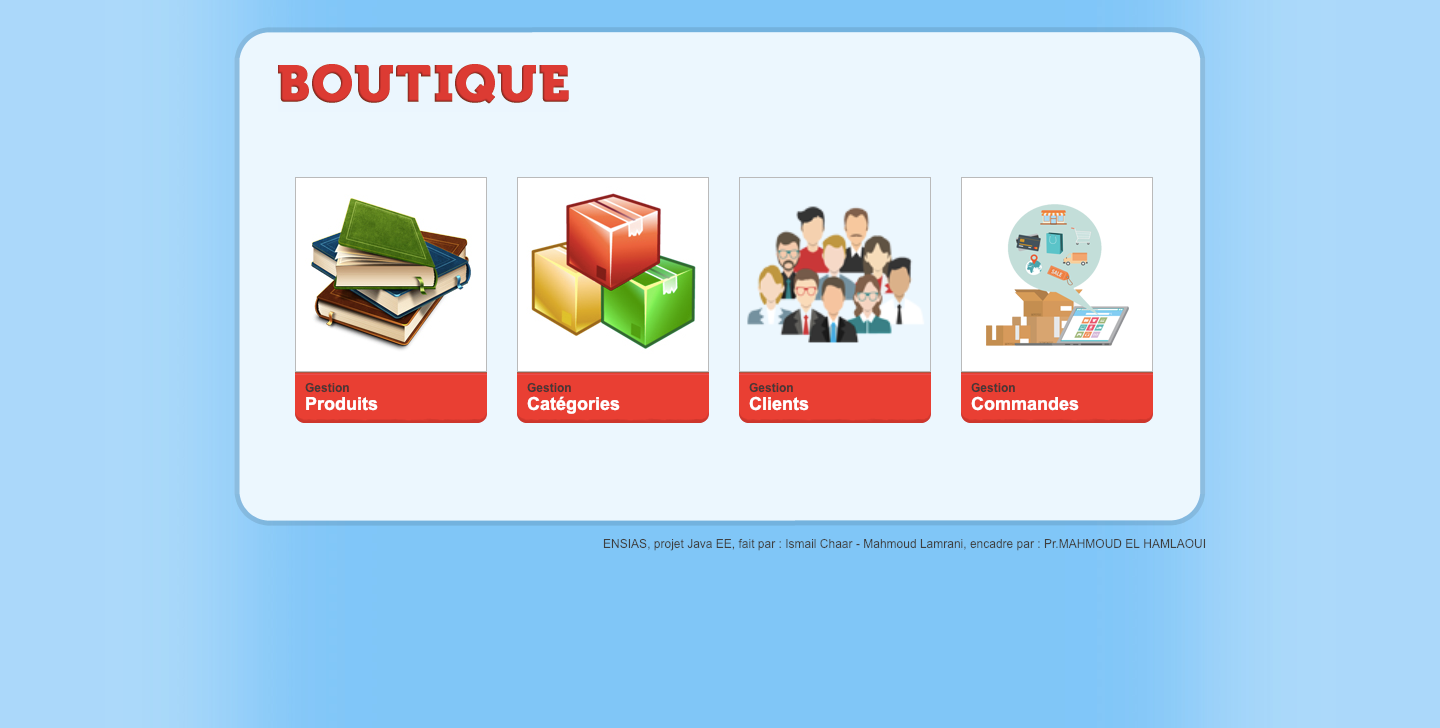
\includegraphics[width=\textwidth,scale=0.8]{screens/Home-Administration.png}}
    \caption{Capture d'écran de la page d'acceuil du BackOffice}
\end{figure}
L'application donne à l'administrateur la possibilité de gérer les livres, les catégories, les clients et les commandes.
\subsubsection{Gestion de livres}
Dans la partie gestion de livres, on a le suivant : 
l'affichage de la liste des livres existants dans l'e-boutique, avec toutes les informations : la première page de couverture, le titre, la catégorie, le prix et la quantité en stock.
La possibilité de supprimer, de modifier un livre ou d'ajouter un nouveau.
\begin{figure}[H]
    \centering
    \fbox{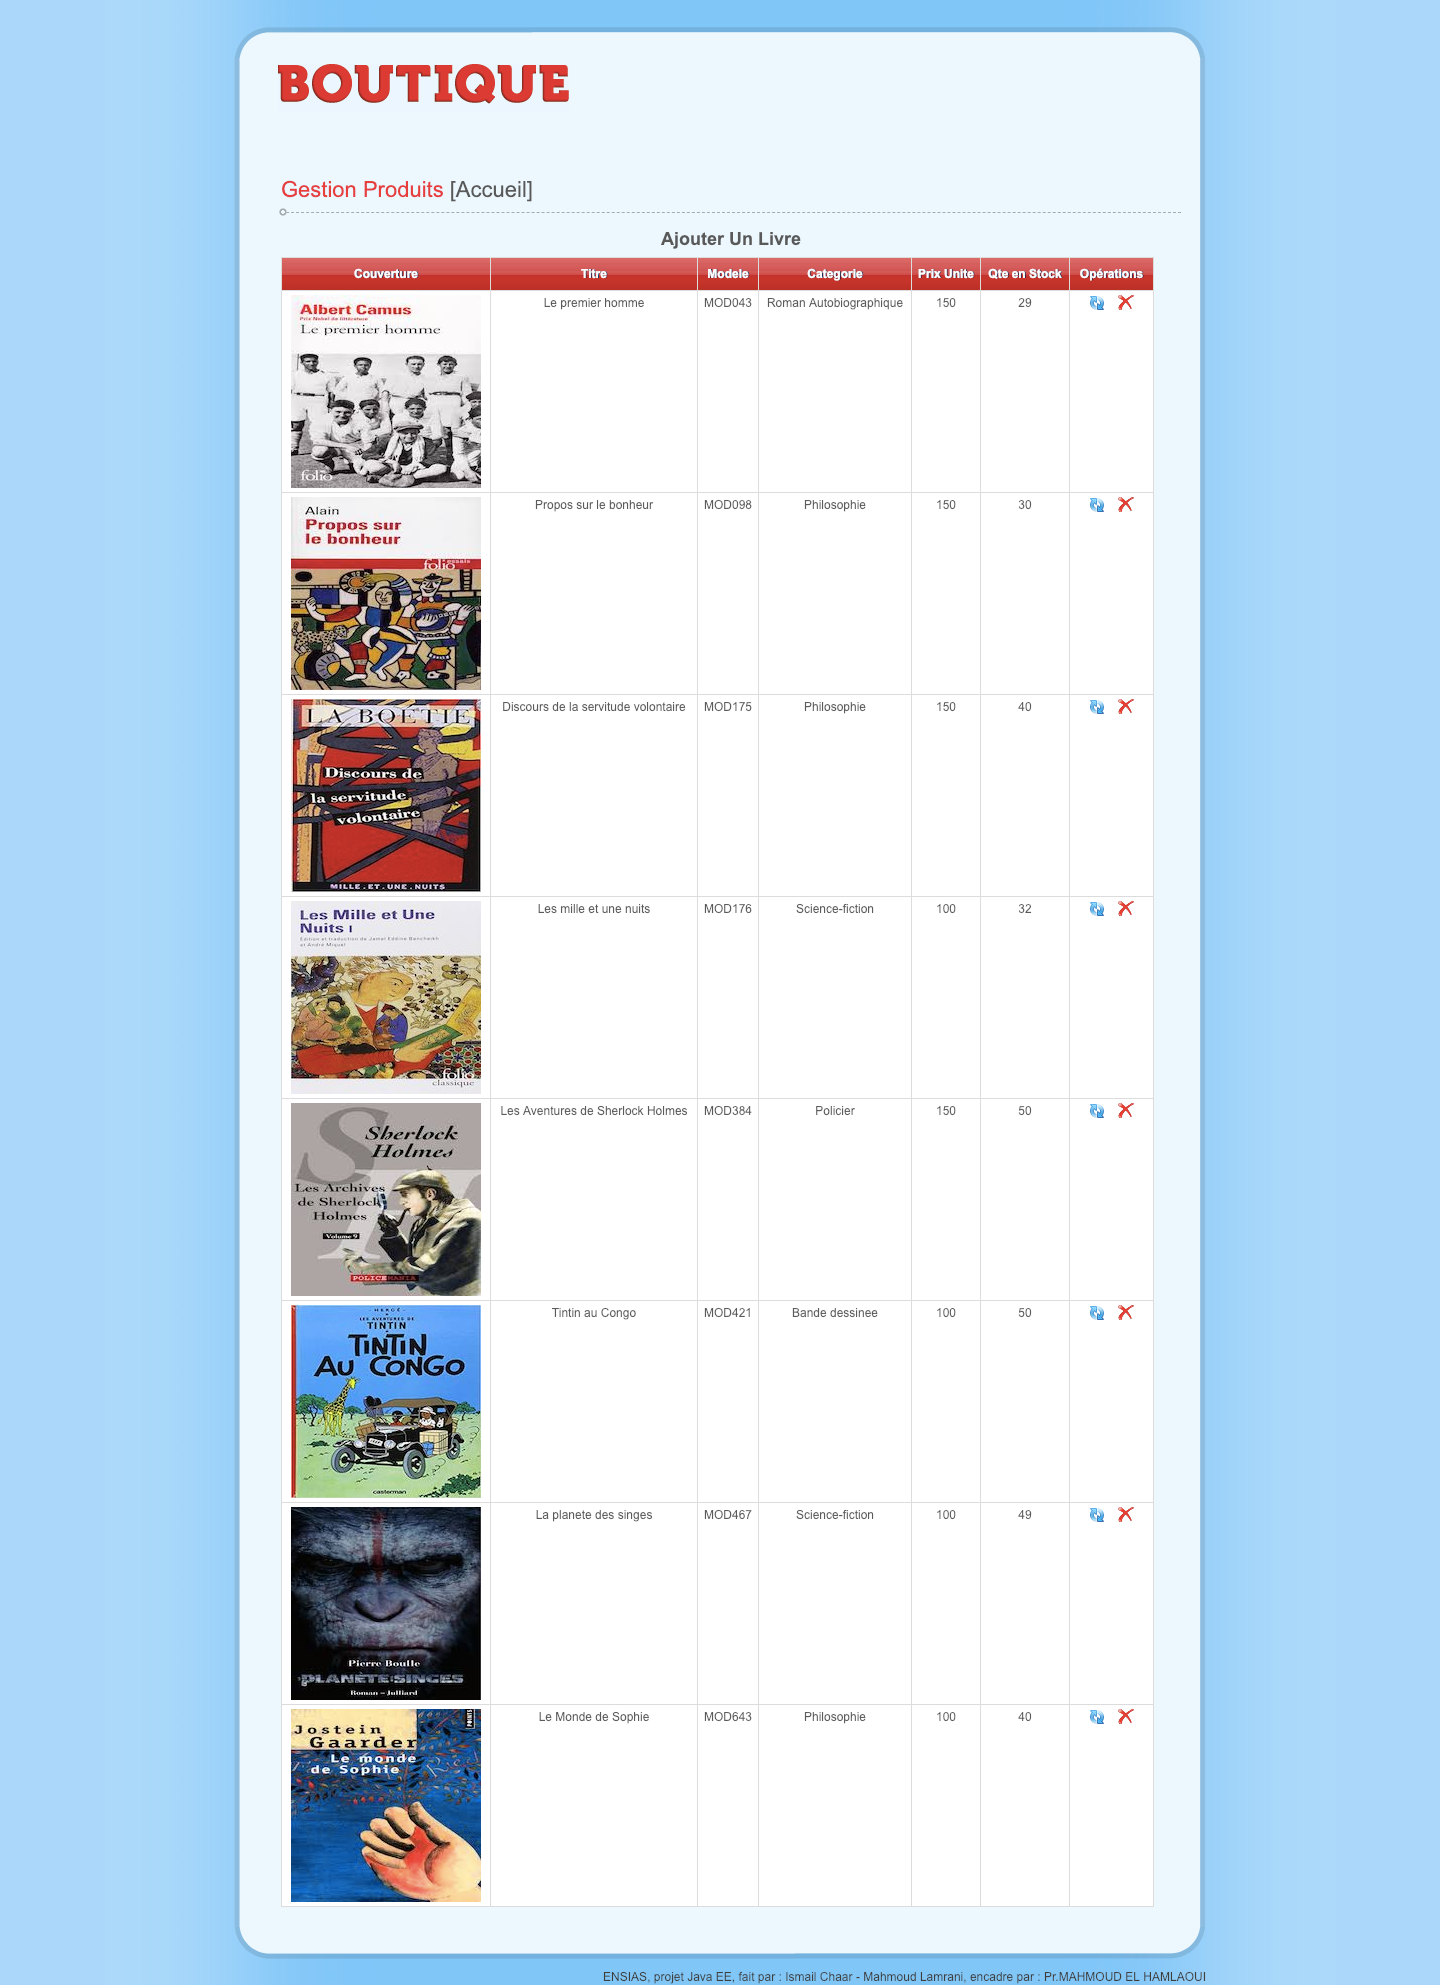
\includegraphics[width=\textwidth,scale=0.75]{screens/GestionProduits.png}}
    \caption{Capture d'écran de la page de gestion de livres}
\end{figure}
\begin{figure}[H]
    \centering
    \fbox{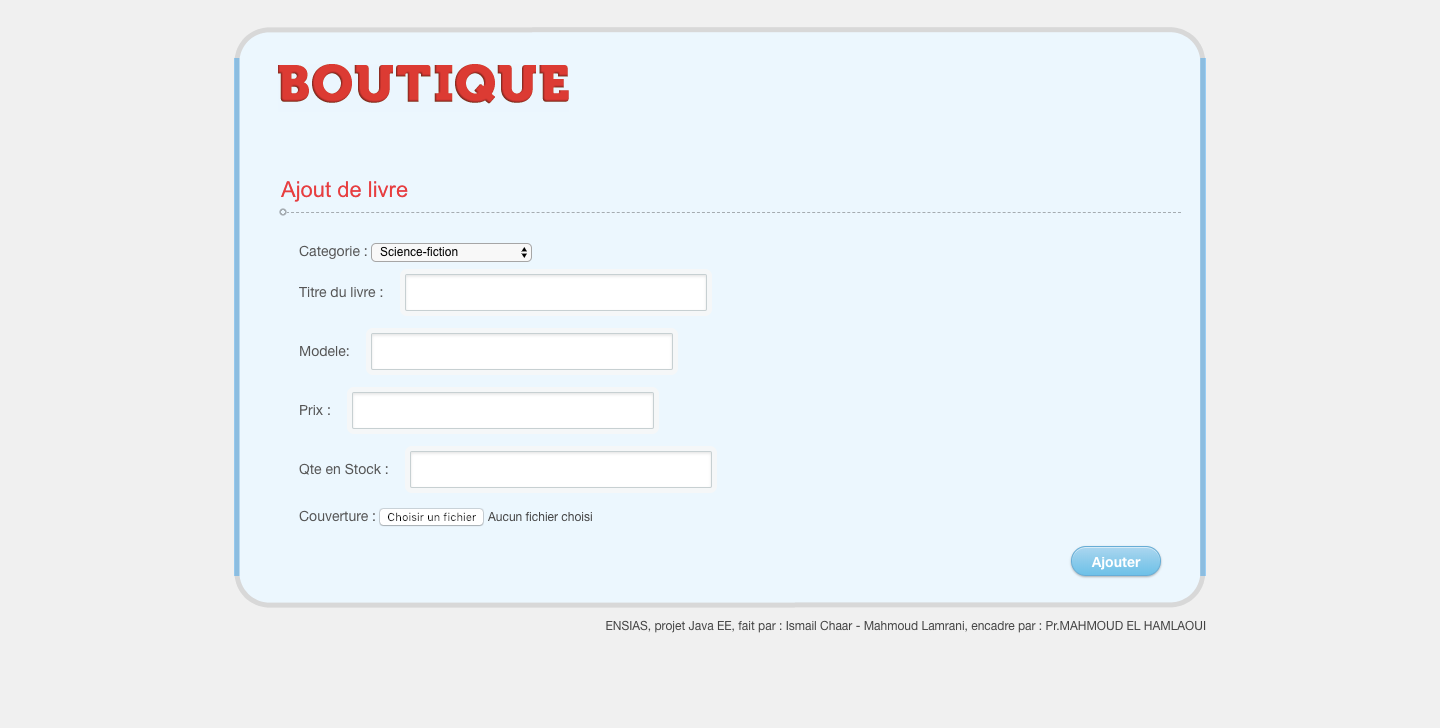
\includegraphics[width=\textwidth,scale=0.8]{screens/AjouterProduit.png}}
    \caption{Capture d'écran de la page d'ajout d'un livre}
\end{figure}
\subsubsection{Gestion de catégories}
Pour les catégories, on affiche toutes les catégories de livres dans le site, on peut soit supprimer une catégorie, modifier son libellé ou bien en ajouter une nouvelle.
\begin{figure}[H]
    \centering
    \fbox{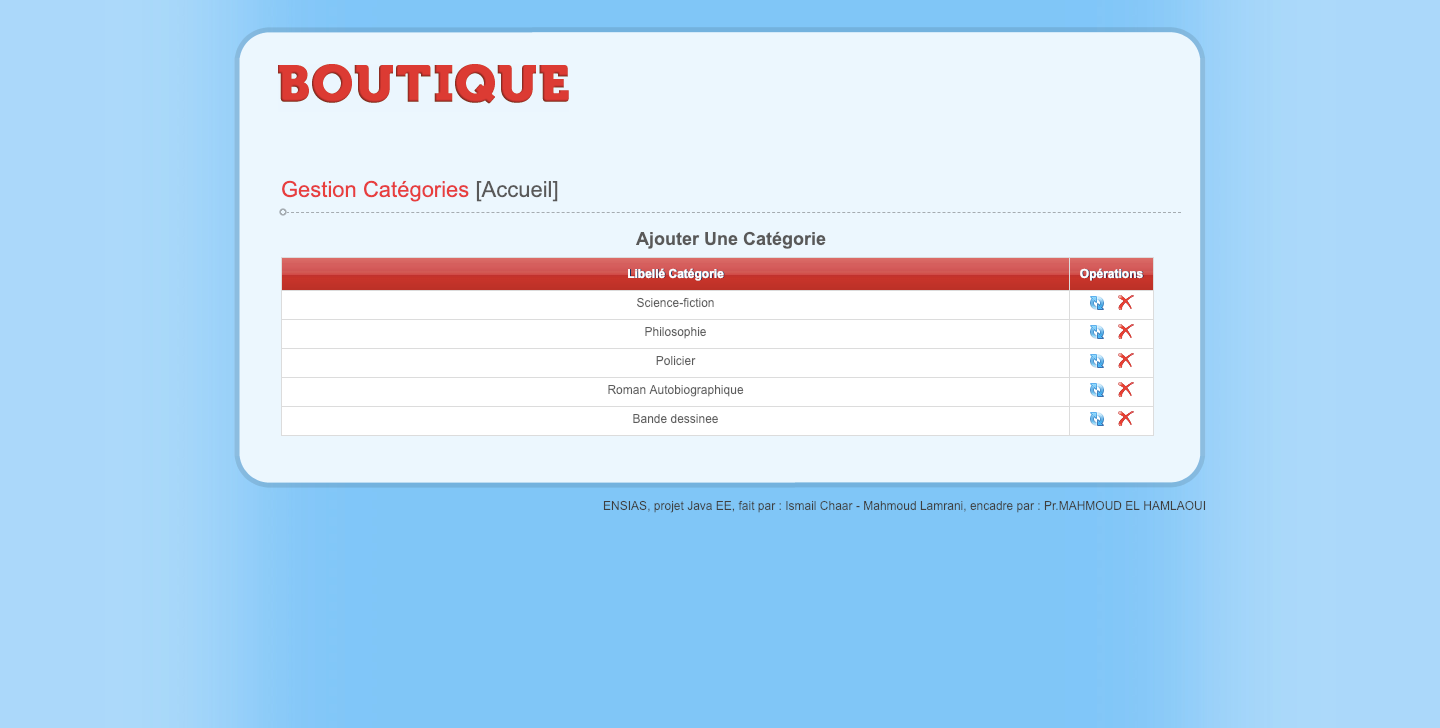
\includegraphics[width=\textwidth,scale=0.8]{screens/GestionCategories.png}}
    \caption{Capture d'écran de la page de gestion de catégories}
\end{figure}
\begin{figure}[H]
    \centering
    \fbox{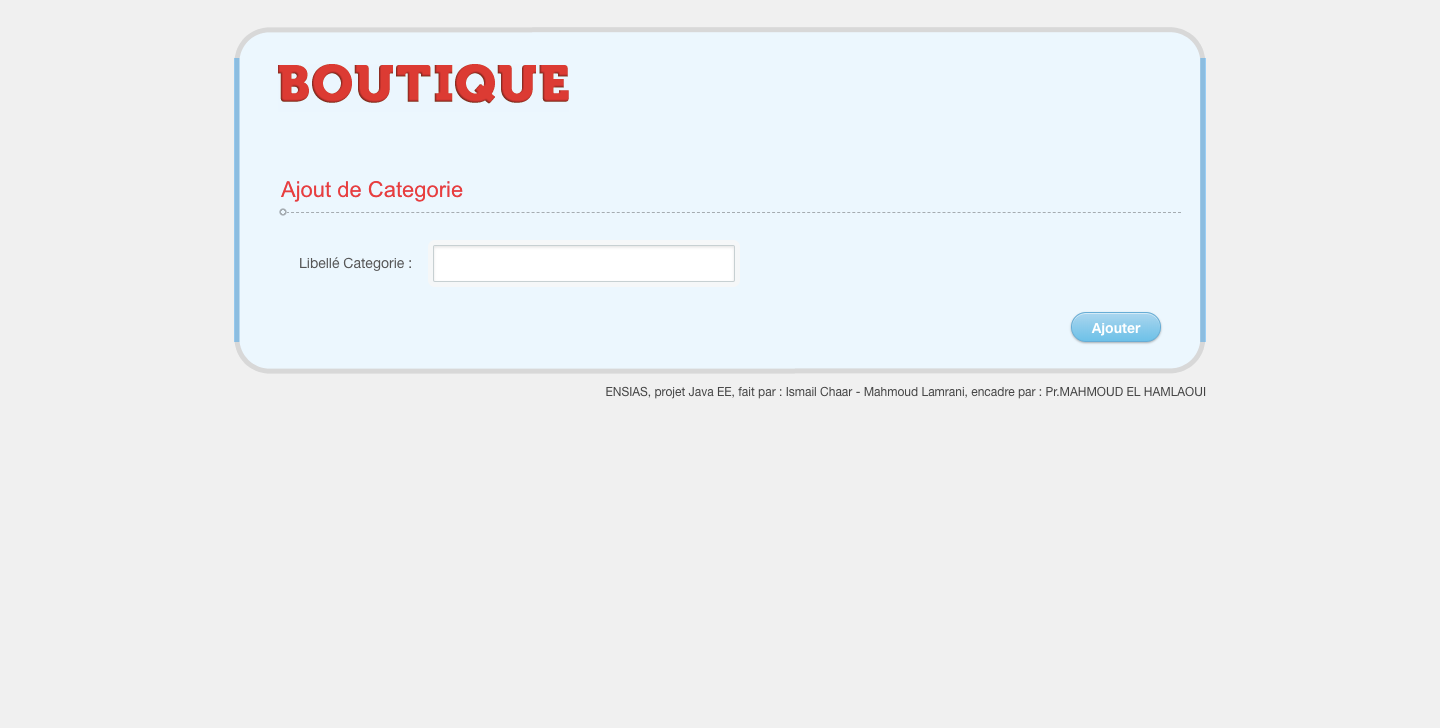
\includegraphics[width=\textwidth,scale=0.8]{screens/AjouterCategorie.png}}
    \caption{Capture d'écran de la page d'ajout d'une catégorie}
\end{figure}
\subsubsection{Gestion de clients}
Pour le volet consacré à la gestion des clients, on affiche les informations de tous les clients de l'e-boutique (nom, adresse, e-mail...) avec la possibilité de supprimer un client.
\begin{figure}[H]
    \centering
    \fbox{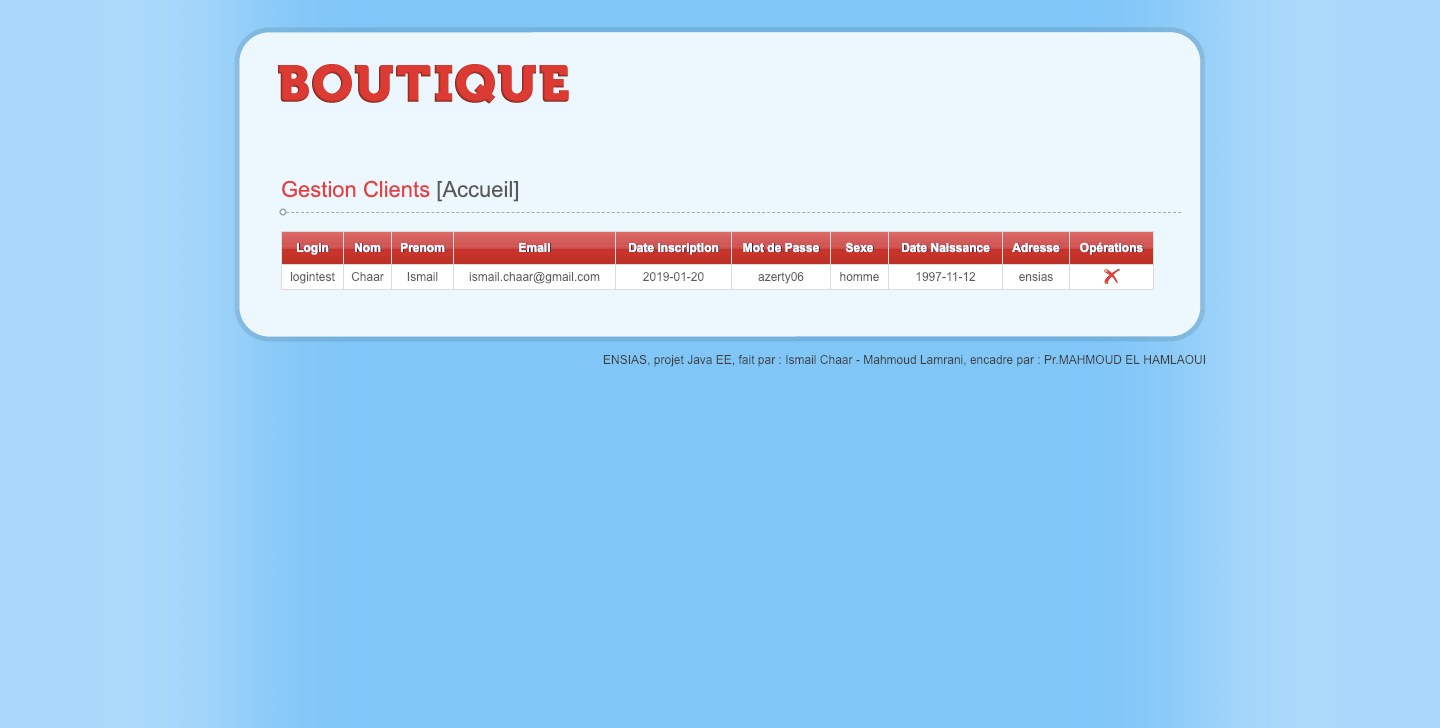
\includegraphics[width=\textwidth,scale=0.8]{screens/GestionClients.png}}
    \caption{Capture d'écran de la page de gestion des clients}
\end{figure}
\newpage
\subsubsection{Gestion de commandes}
On affiche toutes les commandes effectuées par les clients du site, leur prix total, ainsi la possibilité de valider ou non une commande.
\begin{figure}[H]
    \centering
    \fbox{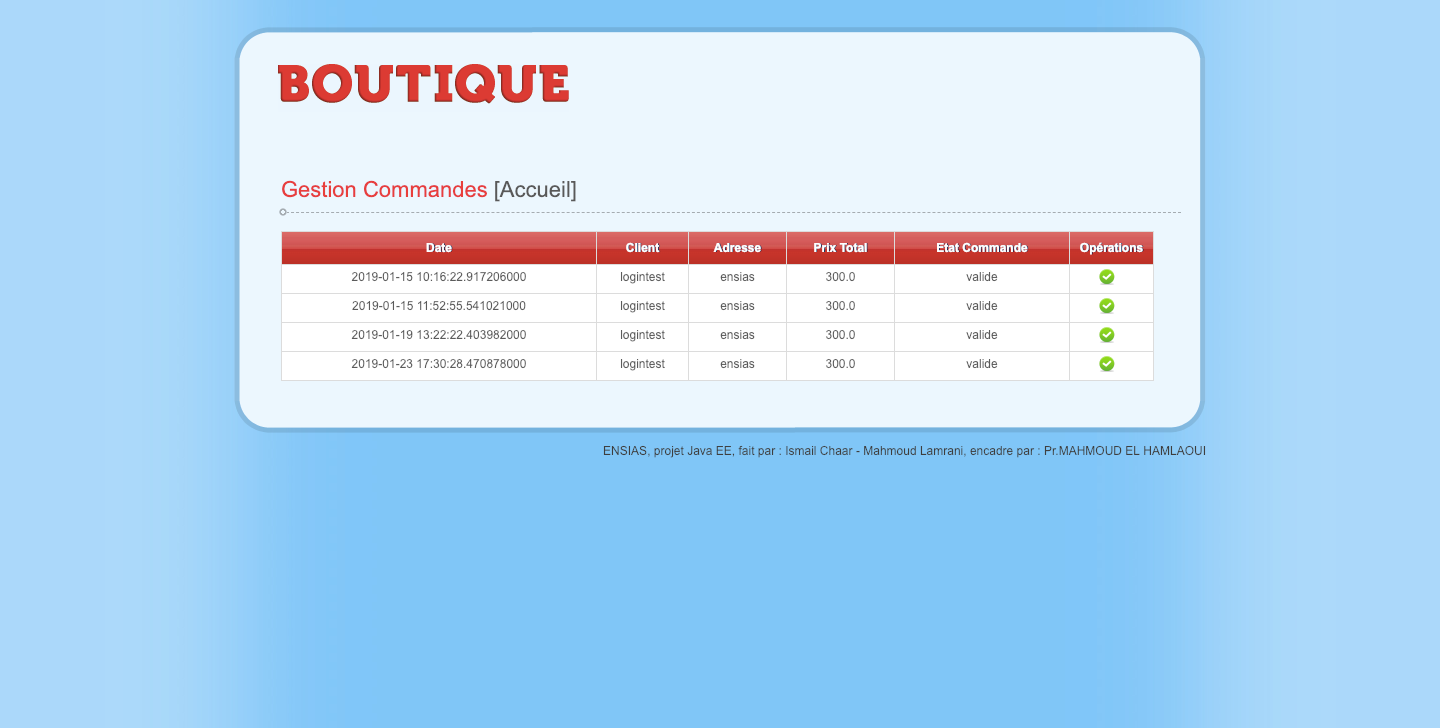
\includegraphics[width=\textwidth,scale=0.8]{screens/GestionCommandes.png}}
    \caption{Capture d'écran de la page de gestion des commandes}
\end{figure}
\subsection{Le FrontOffice}
Le front office est la partie d'un site internet qui est visible par les internautes, celle que l’on consulte et que l’on atteint par l’adresse internet (URL)
\subsubsection{L'acceuil}
Ceci est la partie d'accueil de notre site, on fait représenter un Slider descriptif de quelques livres, on affiche les différentes catégories des livres de l'e-boutique et on montre les nouveaux livres ajoutes à l'e-boutique sous la rubrique Nouvel Arrivage.
\begin{figure}[H]
    \centering
    \fbox{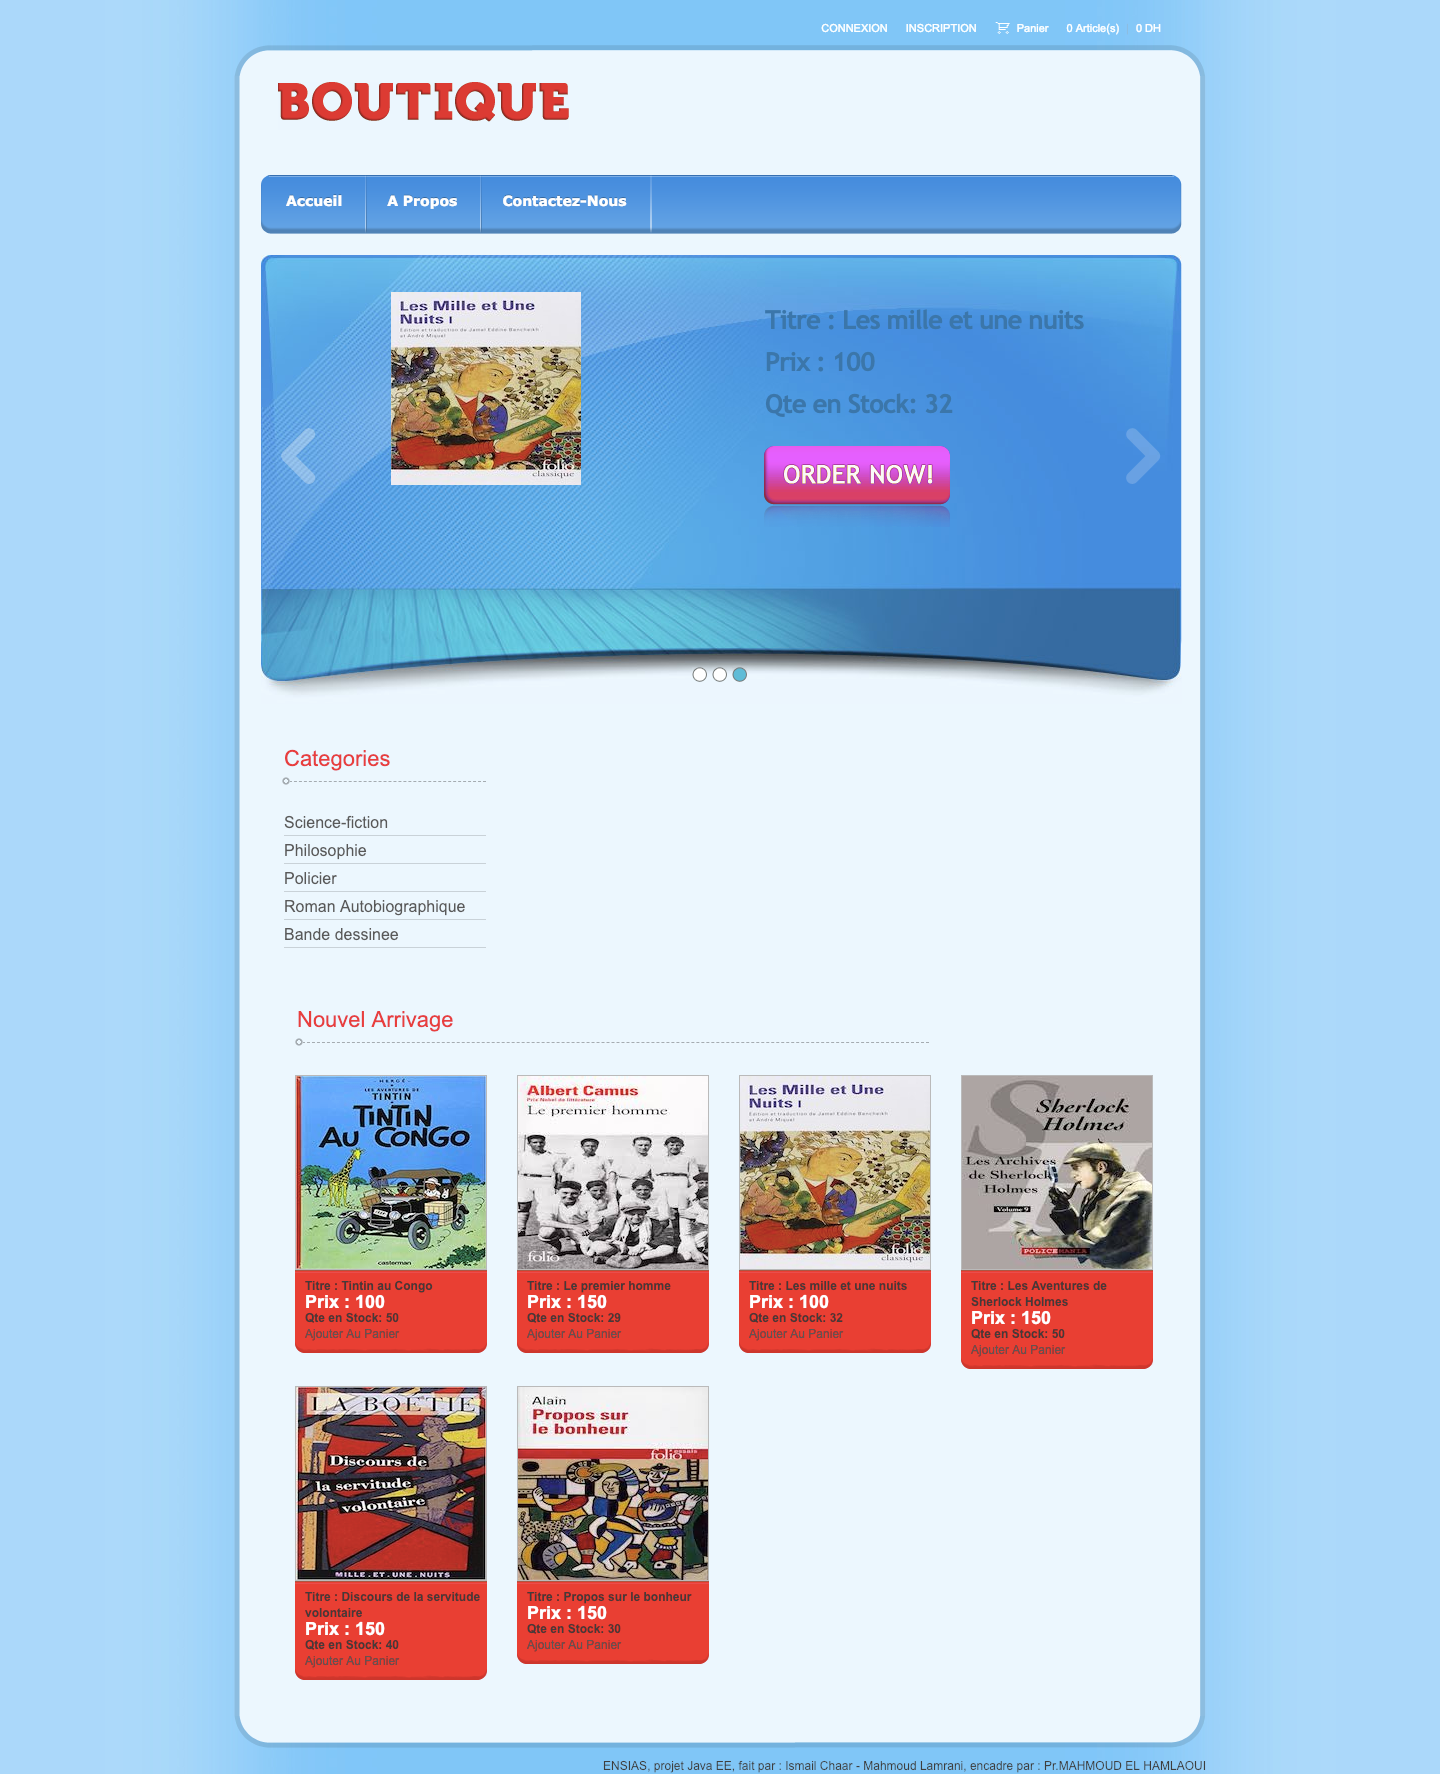
\includegraphics[width=\textwidth,scale=0.8]{screens/Home-Client.png}}
    \caption{Capture d'écran de la page d'acceuil du FrontOffice}
\end{figure}
\newpage
\subsubsection{Authentification}
Pour l'authentification, le client a la possibilité de se connecter s'il a déjà un compte via le formulaire de connexion ou bien de créer un nouveau compte en donnant quelques informations demandées via le formulaire d'inscription.
\begin{figure}[H]
    \centering
    \fbox{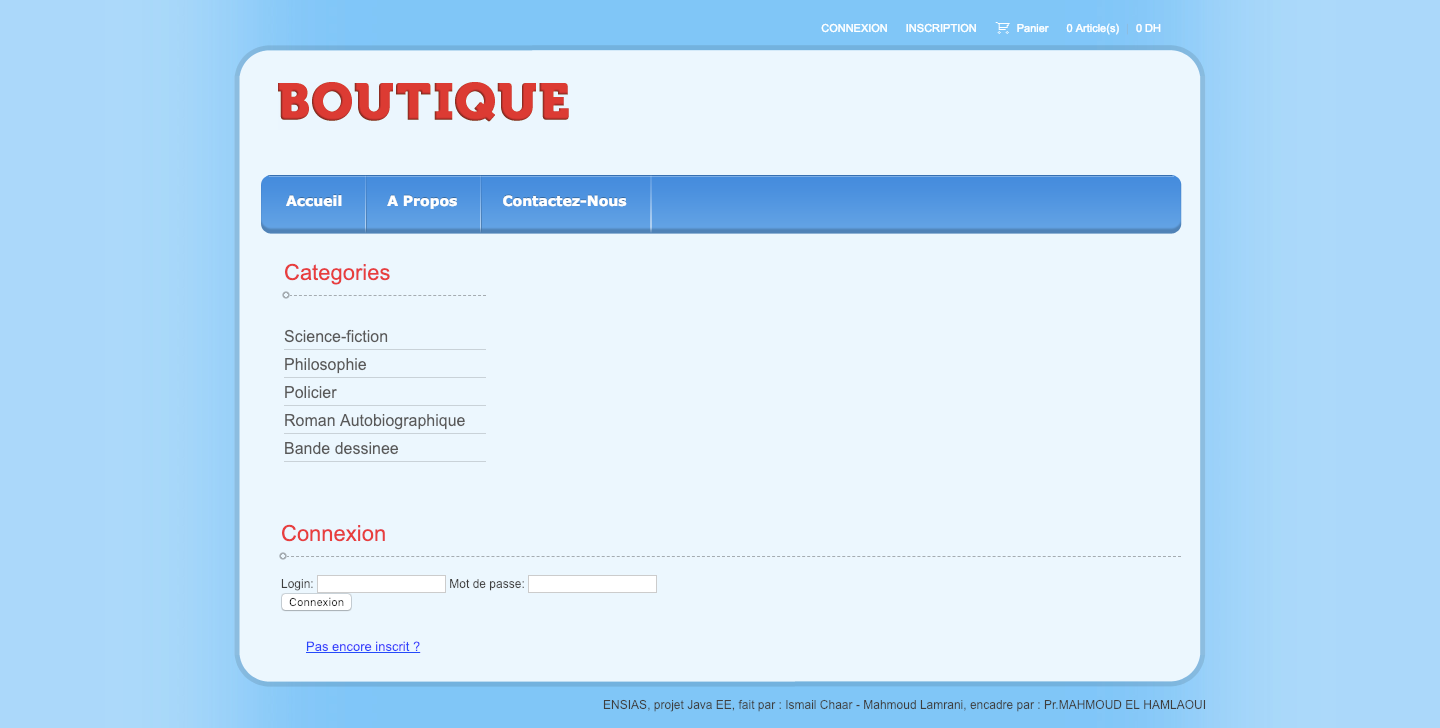
\includegraphics[width=\textwidth,scale=0.8]{screens/connexion.png}}
    \caption{Capture d'écran de la page de connexion}
\end{figure}
\begin{figure}[H]
    \centering
    \fbox{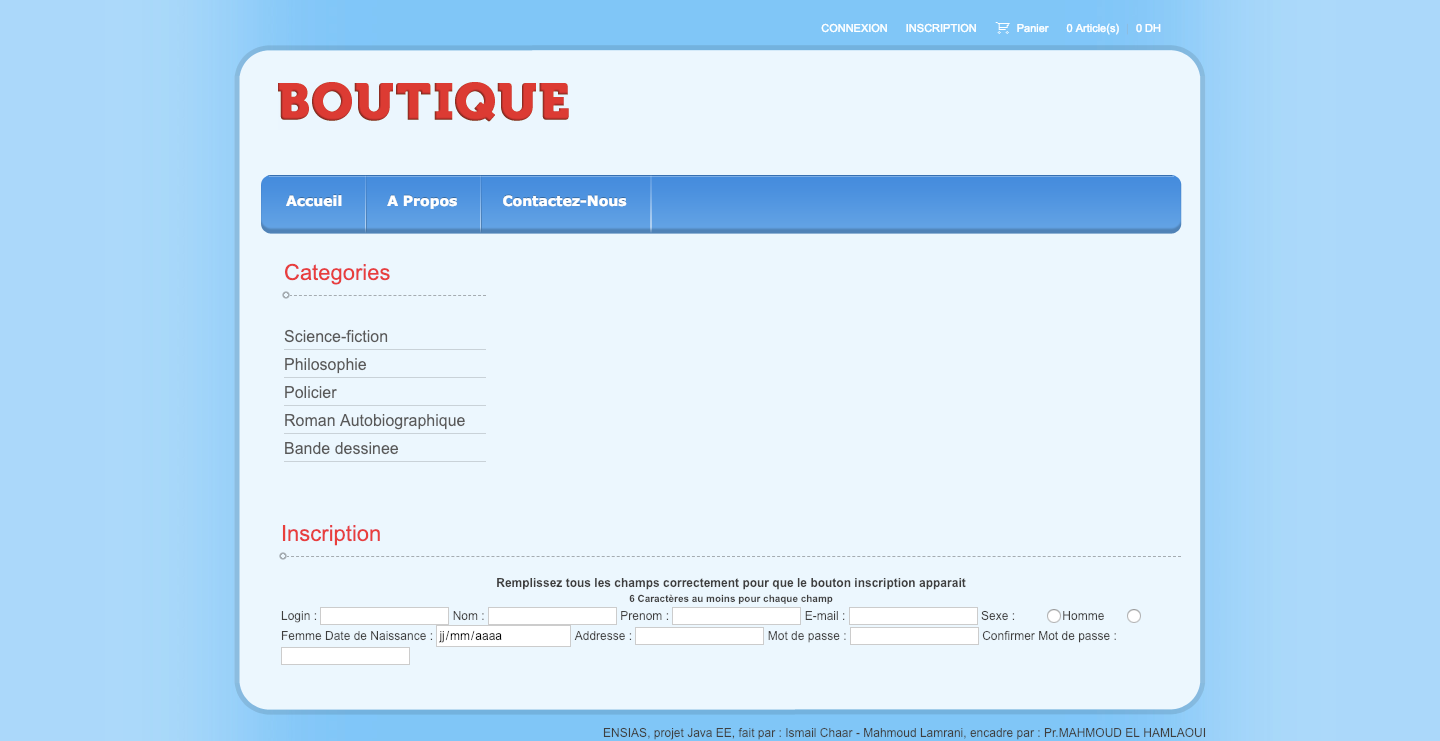
\includegraphics[width=\textwidth,scale=0.8]{screens/Inscription.png}}
    \caption{Capture d'écran de la page d'inscription}
\end{figure}
\newpage
\subsubsection{Panier}
Après avoir sélectionné un livre la page du panier s’ouvre, le client aura trois possibilités de soit cliquer sur « poursuivre les achats » pour choisir d’autres produits, soit cliquer sur « Passer la commande » pour effectuer son achat, soit cliquer sur « enregistrer le panier » pour avoir la possibilité de continuer son achat même après déconnexion.
\begin{figure}[H]
    \centering
    \fbox{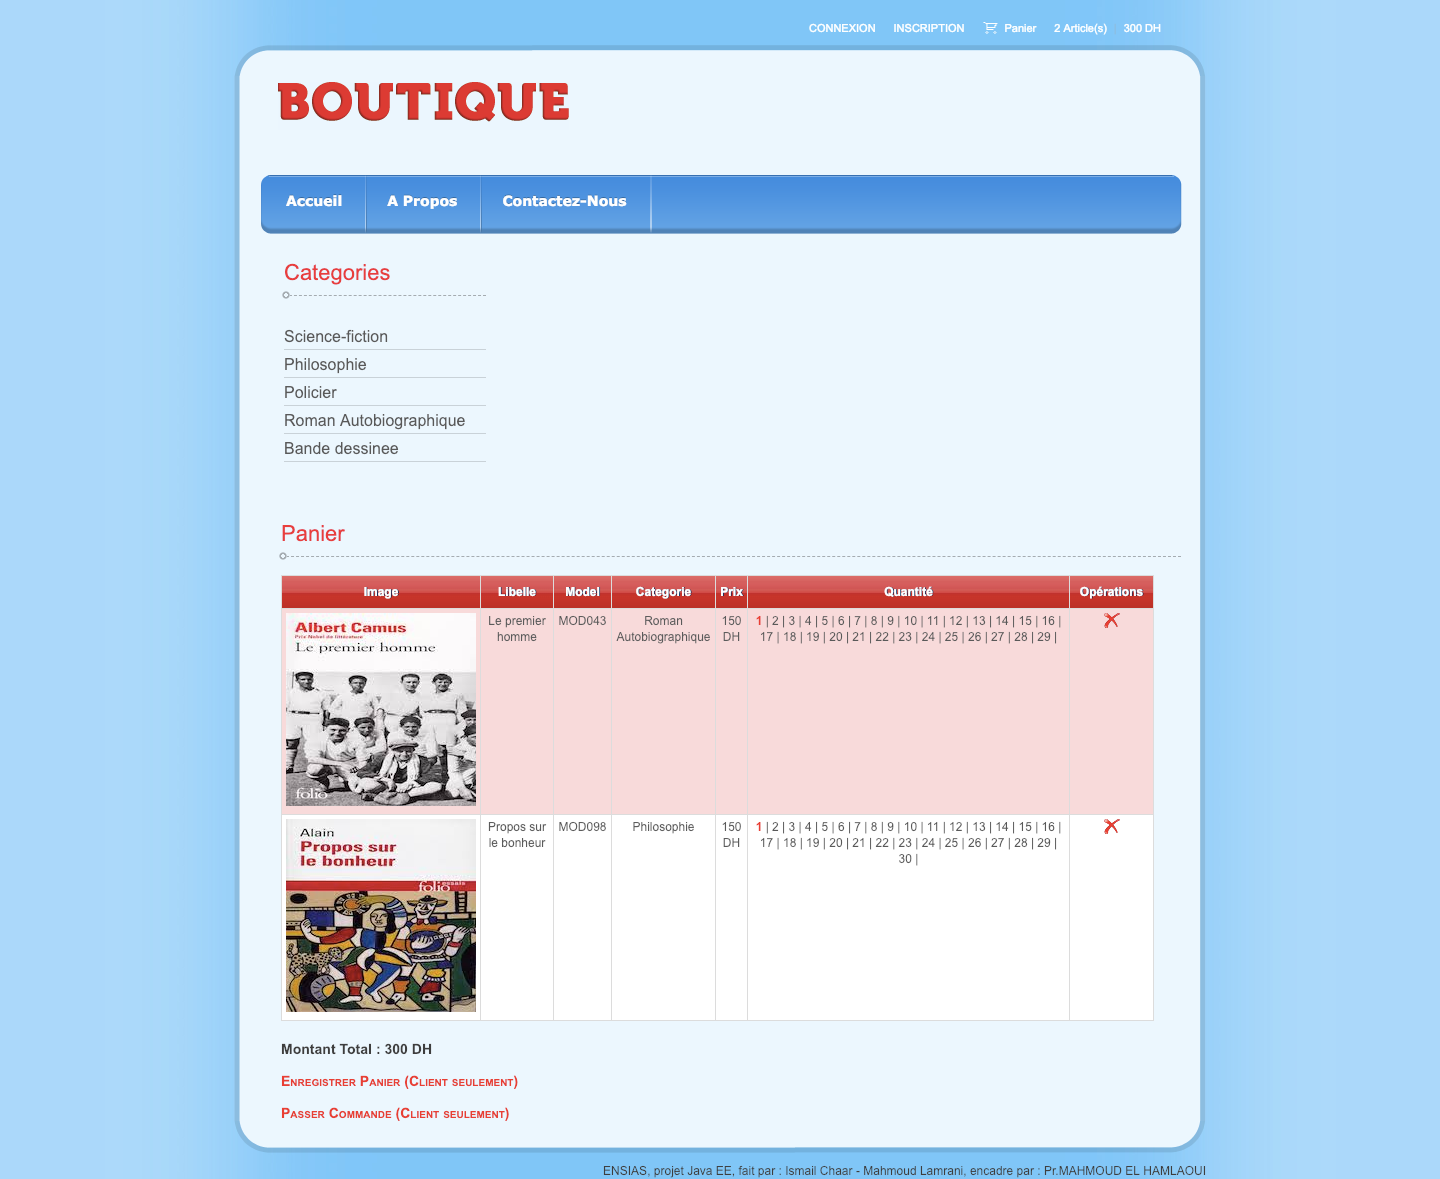
\includegraphics[width=\textwidth,scale=0.8]{screens/Panier.png}}
    \caption{Capture d'écran de la page du panier}
\end{figure}
\newpage
\subsubsection{Espace client}
L'espace client affiche au client ses propres informations, ses commandes et son panier enregistré.
\begin{figure}[H]
    \centering
    \fbox{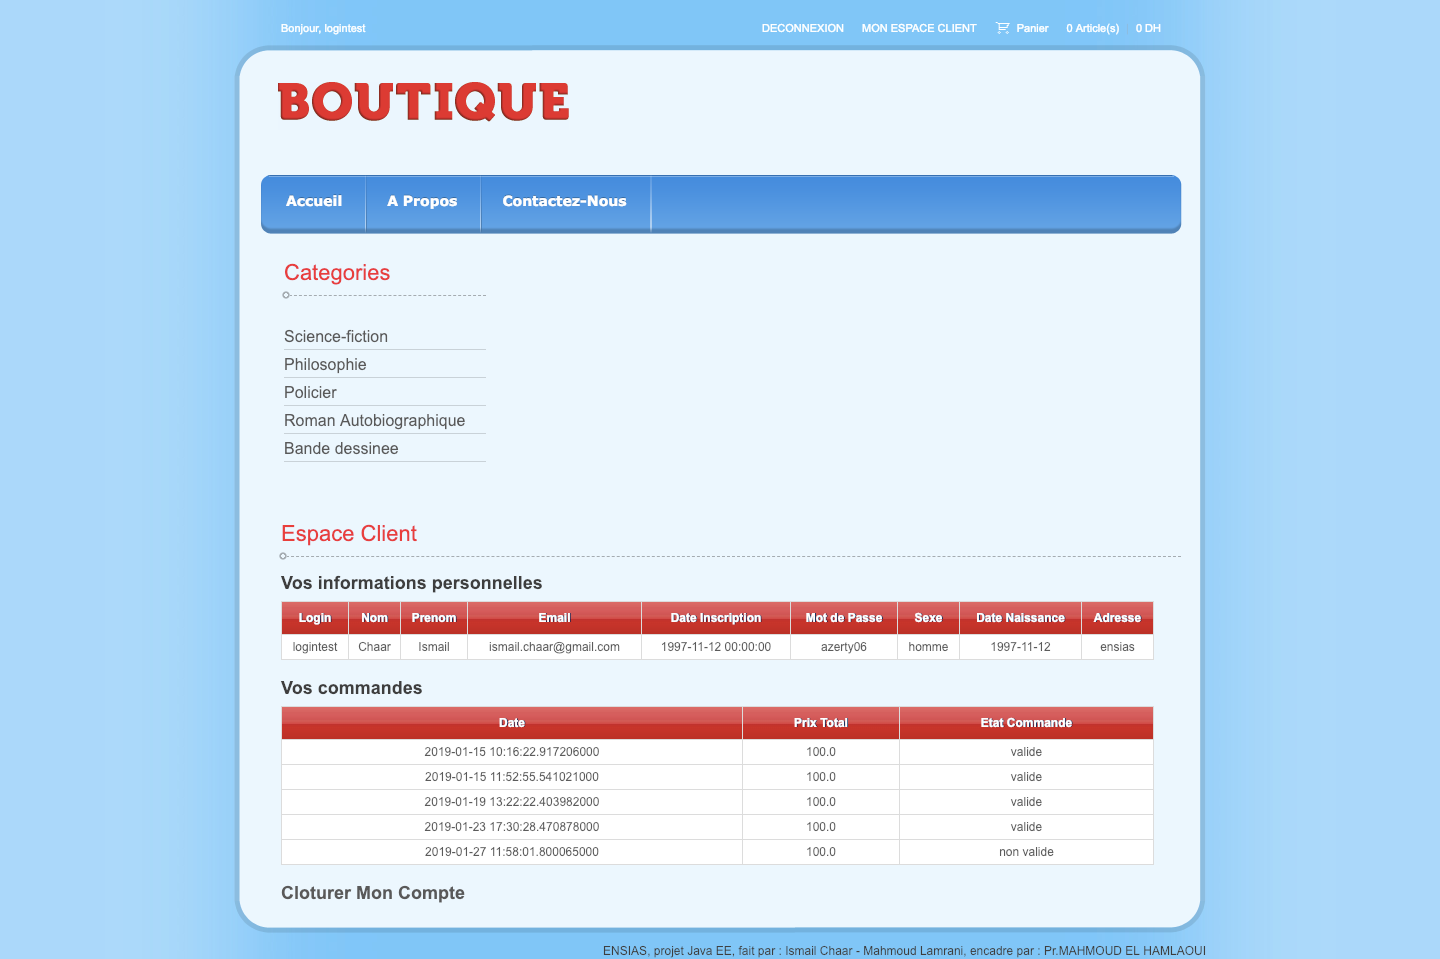
\includegraphics[width=\textwidth,scale=0.8]{screens/Espaceclient.png}}
    \caption{Capture d'écran de la page de l'espace client}
\end{figure}



\input{./autre_partie.tex}





\chapter{Conclusion }
\addcontentsline{toc}{section}{Conclusion }


En réalisant un projet de vente à distance, on a permis au consommateur, en dehors des lieux habituels de réception de la clientèle, d'effectuer sa commande. Cela était possible grâce aux connaissances acquises durant notre formation a l'ENSIAS.
\newline
L’utilisation de l'UML nous a permis d’effectuer une analyse détaillée de l'e-boutique de livre. Ainsi, nous avons pu parfaire nos compétences en termes d’analyse et de conception.
L'utilisation des Javabeans et des DAO s'avérait indispensable pendant la rédaction du code.
\newline
Au niveau de la gestion du projet en binôme, nous avons réussi à bien nous répartir les tâches afin de réaliser nos objectifs dans le temps qu'on avait, Github était incontournable en ce qui concerne ce volet.
En guise de perspectives, il serait intéressant d’ajouter des modes de paiement à notre application web e-boutique de livre comme Paypal et cartes bancaires.

\listoffigures

\newpage

%récupérer les citation avec "/footnotemark"
\nocite{*}

%choix du style de la biblio
\bibliographystyle{plain}
%inclusion de la biblio
\bibliography{bibliographie.bib}
%voir wiki pour plus d'information sur la syntaxe des entrées d'une bibliographie

\end{document}